\documentclass[conference]{IEEEtran}
\IEEEoverridecommandlockouts
% The preceding line is only needed to identify funding in the first footnote. If that is unneeded, please comment it out.
\usepackage{cite}
\usepackage{amsmath,amssymb,amsfonts}
\usepackage{algorithmic}
\usepackage{graphicx}
\usepackage{textcomp}
\usepackage{xcolor}
\usepackage{blindtext}
\usepackage[hidelinks]{hyperref}
\usepackage{booktabs}
\def\BibTeX{{\rm B\kern-.05em{\sc i\kern-.025em b}\kern-.08em
    T\kern-.1667em\lower.7ex\hbox{E}\kern-.125emX}}

\begin{document}
\title{COVID-19: Death Statistical Analysis}
\author{\IEEEauthorblockN{ Aleksei Luchinsky }
\IEEEauthorblockA{\textit{Department of Mathematics and Statistics} \\
\textit{Bowling Green State University}\\
Bowling Green, Ohio \\
aluchi@bgsu.edu}
\and
\IEEEauthorblockN{ Michael Terry}
\IEEEauthorblockA{\textit{Department of Computer Science} \\
\textit{Bowling Green State University}\\
Bowling Green, Ohio \\
mterry@bgsu.edu}
\and
\IEEEauthorblockN{ Vagish Vela}
\IEEEauthorblockA{\textit{Department of Computer Science} \\
\textit{Bowling Green State University}\\
Bowling Green, Ohio \\
vvela@bgsu.edu}
}
\maketitle

\begin{abstract}
Identifying the impact of COVID-19 comparing to historical mortality rates is important to determining the hidden costs of the pandemic not immediately attributable to the disease. 
Determining excess mortality will inform policy-makers in the proper decisions regarding quarantine orders and service shutdowns.
In this paper, we study the impact of COVID-19 on several US states and how the disease compares with historical causes of death and it's potential contribution to excess deaths when compared to an equivalent historical time frame.
%In the long term, the outcomes of this study will be used to support research into: (1) comparing COVID-19 disease statistics between US States. (2) comparing COVID-19 death statistics with historical top causes of death (3) determining the impact of COVID-19 on excess mortality rates as a result of state mandated quarantine measures. 
We provide insights into how our data can support excess death analysis in the future, and reflect on the significant challenges, highlighted by our study, for future research in comparing COVID-19 datasets.
\end{abstract}

\section{Introduction}

Coronavirus Disease 2019 (COVID-19) is a global pandemic since March 2020, as declared by the World Health Organization \cite{cucinotta_who_2020}.
COVID-19 is a major issue in 2020 with significant impact to global economies, as well as the mental and physical health of people worldwide.
Our research seeks to identify trends between US states for COVID-19, and compare it to other causes of death.

Our contributions are comparisons between states focusing on case counts and death counts with a process replicable to all states of the USA. 
Additionally, providing a comparison between each states COVID-19 deaths against other causes of death.
This is also replicable across all states of the USA.
Replication is key in our analysis, and one merely has to pre-process the data into the relevant format and it will run through the analysis.

This paper will focus on a subset of US states: including Ohio, Michigan, Indiana and California with the ability to replicate across all states within the USA.
We have two research questions, the first focuses on comparisons between the states and the second on the comparisons between causes of death:

\textbf{RQ1: Are there similarities with COVID-19 spread between states?} Are the states in the Midwest similar? Also are there differences with states in the south versus the north? We will focus on Indiana, Michigan and Ohio in the Midwest for the first comparison. Then look at California against the Midwest for the second comparison.

\textbf{RQ2: How does COVID-19 compare to other causes of death?} Leveraging the CDC data on excess deaths we will compare COVID-19 against other causes \cite{cdc_weekly_nodate}.


The paper as organized as follows, section II covers the background which focuses on the datasets we use as well as previous work done with those datasets.
Methodology of how we cleaned, processed and analyzed the data is discussed in Section III.
Section IV focuses on the results and discussion of those results.
In section V the results of our work are summarized.

\section{Background}

We utilize data publicly available from Department of Health organizations of each chosen state.
The Ohio data is from the Ohio Department of Health \cite{system_covid-19_nodate}.
The Michigan data is from the State of Michigan \cite{noauthor_coronavirus_nodate}.
The Indiana data is from Indiana State Department of Health (ISDS) \cite{noauthor_indiana_nodate}.
The California data is from California Department of Public Health \cite{noauthor_tracking_nodate}.

Considerable research has been done related to COVID-19. It is still early for extensive, deep research since it takes years for such papers to come out.
Research has been conducted into excess mortality and testing in Ohio \cite{quast_excess_2020}.
The way the virus spread in Amish country in Ohio has been looked at \cite{ali_covid-19_2020}.
There was rapid spread of cases in nursing homes, from the beginning of the pandemic through to mid June ``over 82\% of all cases in the state coming from 37\% of nursing homes'' \cite{bowblis_prevalence_2020}.

There was a decline in stroke victims through the pandemic, which gives us insight into the impact of COVID-19 on other causes of death \cite{uchino_decline_2020}.
Research into potential under-reporting of COVID-19 related deaths, as well as indirect deaths from Stay At Home orders has been looked into \cite{woolf_excess_2020}.
There has been comparative studies into the geographical differences between the states and COVID-19 cases and deaths, specifically looking at estimating incidence rates \cite{cdc_covid-19_response_team_geographic_2020}. 
Along those lines there have been estimations of excess deaths from March to May \cite{weinberger_estimation_2020}, and March to July \cite{woolf_excess_2020-1}.
There has been a lot of research into COVID-19, comparisons between states, predicting spread and looking at excess deaths. 
Much of this research occurred earlier in the year. By comparison, our research examines COVID-19 data from March to December giving us larger datasets to draw on and analyze.

\section{Methodology}

Our methodology is similar for each state. Differences in individual state-supplied raw data requires the use of different techniques in order to transform the data into a standardized format.
For example, some state data was cumulative, while others were daily and sometimes in the case of Ohio by batch (multiple entries per day based on when the data arrived).

We preprocess the data for each state since they are different in their raw formats.
Two processed datasets are created per state.
The first processed dataset is on the county level, with the following columns:
\begin{itemize}
  \item Date - Date of COVID-19 event
  \item State - State it happened in
  \item County - The county within that state
  \item Cases - Daily cases on the specific date within the county
  \item Deaths - Daily deaths on the specific date within the county
\end{itemize}

The second processed dataset is on the state level, with the following columns:
\begin{itemize}
  \item Date - Date of COVID-19 event
  \item State - State it happened in
  \item Cases - Daily cases on the specific date within the state
  \item Positive - Daily positive tests on the specific date within the state
  \item Negative - Daily negative tests on the specific date within the state
  \item Deaths - Daily deaths on the specific date within the state
\end{itemize}

Once preprocessed, the data is imported into our main notebook where each state dataset goes through the same analysis; comparing against the COVIDTracking Project by the Atlantic to compare the numbers from the state and the aggregated numbers by this third party for similarity \cite{covid19tracking_covid_nodate}.
% We look at the statistics of death, and rank COVID-19 fatalities against the other causes of death by state.
% We also examine the population shift by state to see if there is any impact when looking at non-COVID-19 causes of death.
% Testing, negative test results and positive test results are compared between the states.

For visual identification of COVID-19 prevalence within a state geographically, we plot total cases and deaths using GeoJSON by leveraging a TopoJSON collection to help maps counties to a map of the state \cite{eldersveld_topojson_nodate}.

\subsection{Ohio}
\label{Ohio}

The Ohio state department of health has followed good data reporting techniques and publishes clean, tidy and very descriptive data. The primary dataset we work with is called "COVID Summary Data" and is found following the link \cite{system_covid-19_nodate}.

	This dataset currently consists of more
        than 150,000 rows and describes all COVID-19 related cases in Ohio beginning Jan 2,2020 through our cutoff date of Nov 18, 2020. We note this dataset consists almost entirely of raw data and is in the long-table format. There are 9 columns in the table in total, representing the following fields:
        \begin{itemize}
        \item County --- County of residence
        \item Age Range
         \item Sex
        \item Onset Date --- Date the illness began. If onset date is unknown, the date associated with the case is used as a substitute for the date of illness onset.
        \item Date of Death --- Date of death. If date of death is unknown, this variable will be listed as “Unknown”.
        \item Admission Date --- Date of hospital admission. If the date is unknown, it will be listed as “Unknown”.
        \item Case count --- Total number of cases that meet the demographic criteria specified in the corresponding row. For example, the number in this cell is the total number of cases in a county, of the given gender, age range, onset date, etc. Each individual is only counted once. This includes both Confirmed or CDC Expanded Case Definition (Probable).
        \item Deaths Due to Illness Count --- Total number of deaths due to illness that meet the criteria in the given row. Each individual is counted once in this dataset. Note: If this cell is “0” and there is a date listed under “Date of Death” this indicates a death that was not considered to be COVID-19 related.
        \item Hospitalized Count --- Sum of hospitalizations that meet the criteria in the given row. Each individual is only counted once in this dataset. Data in this cell is cumulative and not the amount of people that are currently hospitalized.
        \end{itemize}
Typical extract from the dataset is shown on table \ref{tab:OhioDS}.


\begin{table*}
  \tiny
  \centering
  \begin{tabular}{lllllllrrr}
\toprule
{} &    County &      Sex & Age Range & Onset Date & Date Of Death & Admission Date &  Case Count &  Death Due to Illness Count &  Hospitalized Count \\
\midrule
49384  &  Hamilton &   Female &       80+ & 2020-11-19 &           NaN &            NaN &           1 &                           0 &                   0 \\
7791   &    Butler &   Female &      0-19 & 2020-11-19 &           NaN &            NaN &           1 &                           0 &                   0 \\
51824  &  Hamilton &     Male &       80+ & 2020-11-19 &           NaN &            NaN &           2 &                           0 &                   0 \\
10993  &    Butler &     Male &       80+ & 2020-11-19 &           NaN &            NaN &           1 &                           0 &                   0 \\
7588   &     Brown &     Male &       80+ & 2020-11-19 &           NaN &            NaN &           1 &                           0 &                   0 \\
7538   &     Brown &     Male &     60-69 & 2020-11-19 &           NaN &            NaN &           1 &                           0 &                   0 \\
7368   &     Brown &     Male &     20-29 & 2020-11-19 &           NaN &            NaN &           1 &                           0 &                   0 \\
7403   &     Brown &     Male &     30-39 & 2020-11-19 &           NaN &            NaN &           1 &                           0 &                   0 \\
14057  &     Clark &     Male &     70-79 & 2020-11-19 &    10/10/2020 &            NaN &           1 &                           1 &                   0 \\
121524 &     Wayne &  Unknown &      0-19 & 2020-11-19 &           NaN &            NaN &           1 &                           0 &                   0 \\
\bottomrule
\end{tabular}
\caption{Extract from Ohio dataset}
\label{tab:OhioDS}
\end{table*}

The dataset is clean. In table \ref{tab:Ohio:missing} number and percentage of the missing data in each row is shown. As you can see, we have only absent data in "Admission Date" and "Date of Deaths" columns (81\% and 95\% respectively). This is not the problem of the dataset and means only that in the majority of the cases the patient was not hospitalized (and the admission date is left blank) and/or is alive (this correspond to undefined "Date of Deaths" field).

\begin{table}
  \centering
  \begin{tabular}{ll}
    \toprule
    Field Name & Missing (\%) \\
    \midrule
    County & 0  \\
    Sex & 0  \\
    Age Range & 0  \\
               Onset Date & 0  \\
               Date Of Death & 95 \\
               Admission Date &  82 \\
               Case Count & 0  \\
               Death Due to Illness Count & 0 \\
               Hospitalized Count & 0  \\
    \bottomrule
  \end{tabular}
  \caption{Missing data in Ohio dataset}
  \label{tab:Ohio:missing}
\end{table}

It was mentioned already, that the dataset is in long-table format, so a lot of information can be extracted from it after some work. For example, it is easy to construct time distributions of the total COVID-19 cases/deaths/hospitalizations, determine the mean time spent in hospital, percentage of people died in hospitals and at home, etc. The other example of the dataset, published by the COVIDTracking Project, is available through the link \cite{covid19tracking_covid_nodate}. The data in this dataset is already processed, so only the projections of the original data (like the one discussed earlier) on different variables are available. This makes it easier to extract some information (like time distributions of the deaths cases), but some other information (the role of age and gender, for example) is lost completely. Later in our report we will compare the results extracted from these two data sets.

The original goal of our project was to study mortality rate due to COVID-19 and compare if with the number of deaths caused by other reasons (natural, cancer, flue, etc). On the Ohio site \cite{statistics_stats_nodate} the yearly statistics for last 4 years is presented with classification by different dearth causes. During our work we extracted this information from the site with the help of python Beautiful Soup package \cite{team_beautiful_nodate}. In table the \ref{tab:mortalityStats} current information from this site is shown. Later we have found that the same information for all states is available also in nice CSV format from the link \cite{cdc_weekly_nodate}. 

\begin{table*}
  \centering
\begin{tabular}{lrrrrr}
\toprule
Year &   2014 &   2015 &   2016 &   2017 &   Mean \\
Cause                             &        &        &        &        &        \\
\midrule
Heart Disease                     &  27000 &  28069 &  27410 &  28008 &  27621 \\
Cancer                            &  25433 &  25396 &  25509 &  25643 &  25495 \\
Accidents                         &   6178 &   6756 &   7999 &   8971 &   7476 \\
Chronic Lower Respiratory Disease &   6765 &   7211 &   7015 &   7312 &   7075 \\
Stroke                            &   5791 &   5945 &   5987 &   6425 &   6037 \\
Alzheimer’s disease               &   4083 &   4643 &   5031 &   5117 &   4718 \\
Drugs                             &   2744 &   3310 &   4329 &   5111 &   3873 \\
Diabetes                          &   3641 &   3645 &   3568 &   3740 &   3648 \\
Flu/Pneumonia                     &   2443 &   2445 &   2187 &   2243 &   2329 \\
Kidney Disease                    &   2002 &   2100 &   2262 &   2237 &   2150 \\
Septicemia                        &   1729 &   1957 &   1995 &   2066 &   1936 \\
\bottomrule
\end{tabular}
\caption{Ohio Mortality from different causes \label{tab:mortalityStats}}
\end{table*}

\subsection{Michigan}

COVID-19 data from Michigan is split into multiple excel files which are timestamped in the name.
The dataset we are working with is from the State of Michigan \cite{noauthor_coronavirus_nodate}.
The data is already summarized into daily data.

To get the data from Michigan we go to their website and download the relevant excel files focused on the files for daily counts and daily testing data \cite{noauthor_coronavirus_nodate}.
Then look at what data is missing, and we found 3 dates are missing and we assume this is due to the cases and deaths that they couldn't attribute to a date. 
The number of cases or deaths on those 3 entries is minimal that we filter them out.
\begin{table}
  \centering
\begin{tabular}{ll}
  \toprule
  Field Name & Missing (\%) \\
  \midrule
  COUNTY            &  0.00 \\
  Date              &  0.02 \\
  CASE\_STATUS       &  0.00 \\
  Cases             &  0.00 \\
  Deaths            &  0.00 \\
  Cases.Cumulative  &  0.00 \\
  Deaths.Cumulative &  0.00 \\
  Updated           &  0.00 \\
  \bottomrule
  \end{tabular}
  \caption{Missing data in Michigan dataset}
  \label{tab:Michigan:missing}
\end{table}

Then we set the appropriate data types so it can be processed effectively, and filter out the probable cases so we can focus on confirmed cases.

The data is now in a preprocessed format and we pass it to the main notebook where the comparisons between states and against other causes of deaths happens.


\subsection{Indiana}

COVID-19 data from Indiana is provided in multiple different datasets. 
One particular dataset contained all relevant pieces of data in time series format for the analysis we are performing.
To get the data from Indiana we go to their website and download the data and dictionary files for COVID-19 County-Wide Test, Case, and Death Trends.
This data is already stored in time series format which saves on aggregation steps.
There is no missing data as of writing this report and the data was in very good format. After reviewing the data, we selected a subset of columns containing only the data we had decided to include in our standardized format. After selection, the data subset was exported in the standardized format for further processing and analysis.

\subsection{California}


COVID-19 data from California is provided in multiple different datasets.
Unfortunately, no one dataset provided all the data we needed for our analysis so we imported 2 datasets: each contains statewide cases and testing result rates respectively.
To get the data from California we go to the department of health website and download the data files for COVID-19 Cases and Tests.
We were unable to locate positive testing data on the health department website so we were forced to use a secondary source from the COVID Tracking Project.
This data is already stored in time series format which saves on aggregation steps.
There is no missing data as of writing this report and the data was in very good format. After reviewing the data, we selected a subset of columns containing only the data we had decided to include in our standardized format. After selection, the data subset was exported in the standardized format for further processing and analysis.

\section{ Results \& Discussion }

The main goal of our project is to study the time dependence of death cases caused by COVID-19 virus pandemic and compare it with the available data about deaths caused by other reasons (such as heart diseases, usual influenza, etc). It could be interesting also to make such an analysis for different States or even counties.

Let us start with the general yearly distributions. Unfortunately we failed to find data on natural causes statistics by county, so only state-wide analysis was performed.. It turns out that for all considered by our group states on yearly scale the COVID-19 virus was not the main cause of death. In the case of the Ohio state, for example, it is in the 6th place, just between Alzheimer decease and strokes. (see figure \ref{fig:yearly_deaths} for more details). Almost the same situation is observed for other analyzed by our group states. In all cases heart diseases are the most important death causes, while deaths caused by COVID-19 virus are on 4-6 place.


\begin{figure}
  \centering
  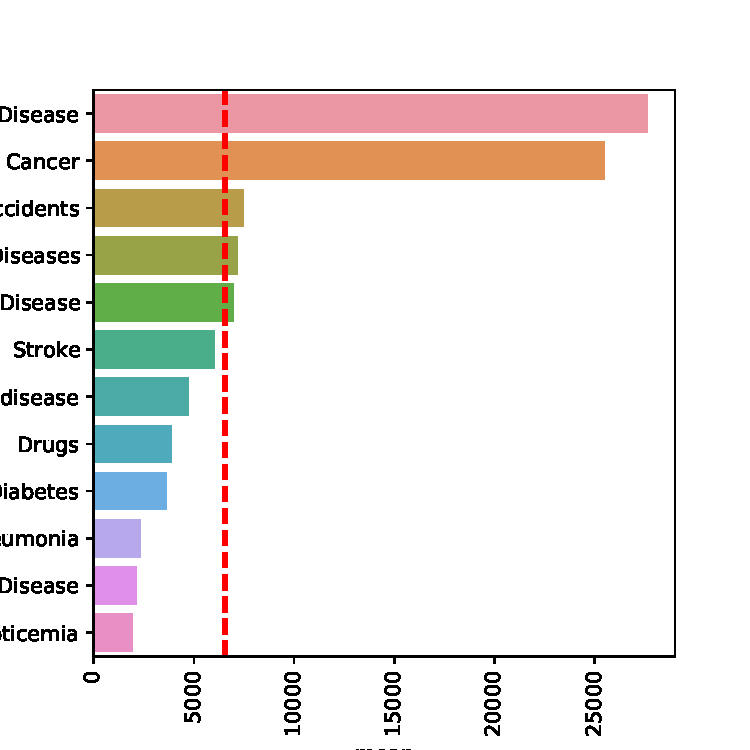
\includegraphics[width=0.9\columnwidth]{figs/yearly_deaths}
  \caption{Comparison}
  \label{fig:yearly_deaths}
\end{figure}


This point is rather interesting and seems to to be very  important. It is clear that because of various precaution measures (such as self isolation, quarantine, lockdown of different industries) the life of the whole world changed dramatically in 2020 year because of COVID-19 a lot of necessary medical procedures were delayed or even canceled, lots of industries were almost bankrupted, etc. Not to mention the most close for us now field, i. e. the education (one can argue about some positive sides of the remote education, but it is definitely different completely from the usual face-to-face process and much more difficult for both students and instructors/professors). Thus, we can say that a lot of money and efforts were lost because of the lockdown during this pandemic and a natural question arises: does it worth it, was is really necessary? As you can see from figure \ref{fig:yearly_deaths}, heart diseases are much more dangerous, but we do not stop the life because of them.



To answer this question it could be interesting to perform a more detailed analysis and study the weekly dependence of the statistics of deaths caused by various deceases. It is clear, that COVID data, collected by our group, gives us a nice opportunity to extract time dependence of death cases with such a granularity (either directly, as for Michigan and Indiana states, or after some obvious transformations, as in the case of raw Ohio data). The same information, actually, in available from COVID Tracking Project \cite{covid19tracking_covid_nodate}, but we decided to work with the original data first. In the left part of figure \ref{fig:RT_comp} we compare time distributions of the deaths cases extracted from the original data and COVID Tracking Project results. From this figure it is clear that for all states under consideration uncumulative distributions are in good agreement, while in the case of shown on the right of the figure \ref{fig:RT_comp} cumulative results the difference is hardly noticeable.

\begin{figure*}
  \centering
  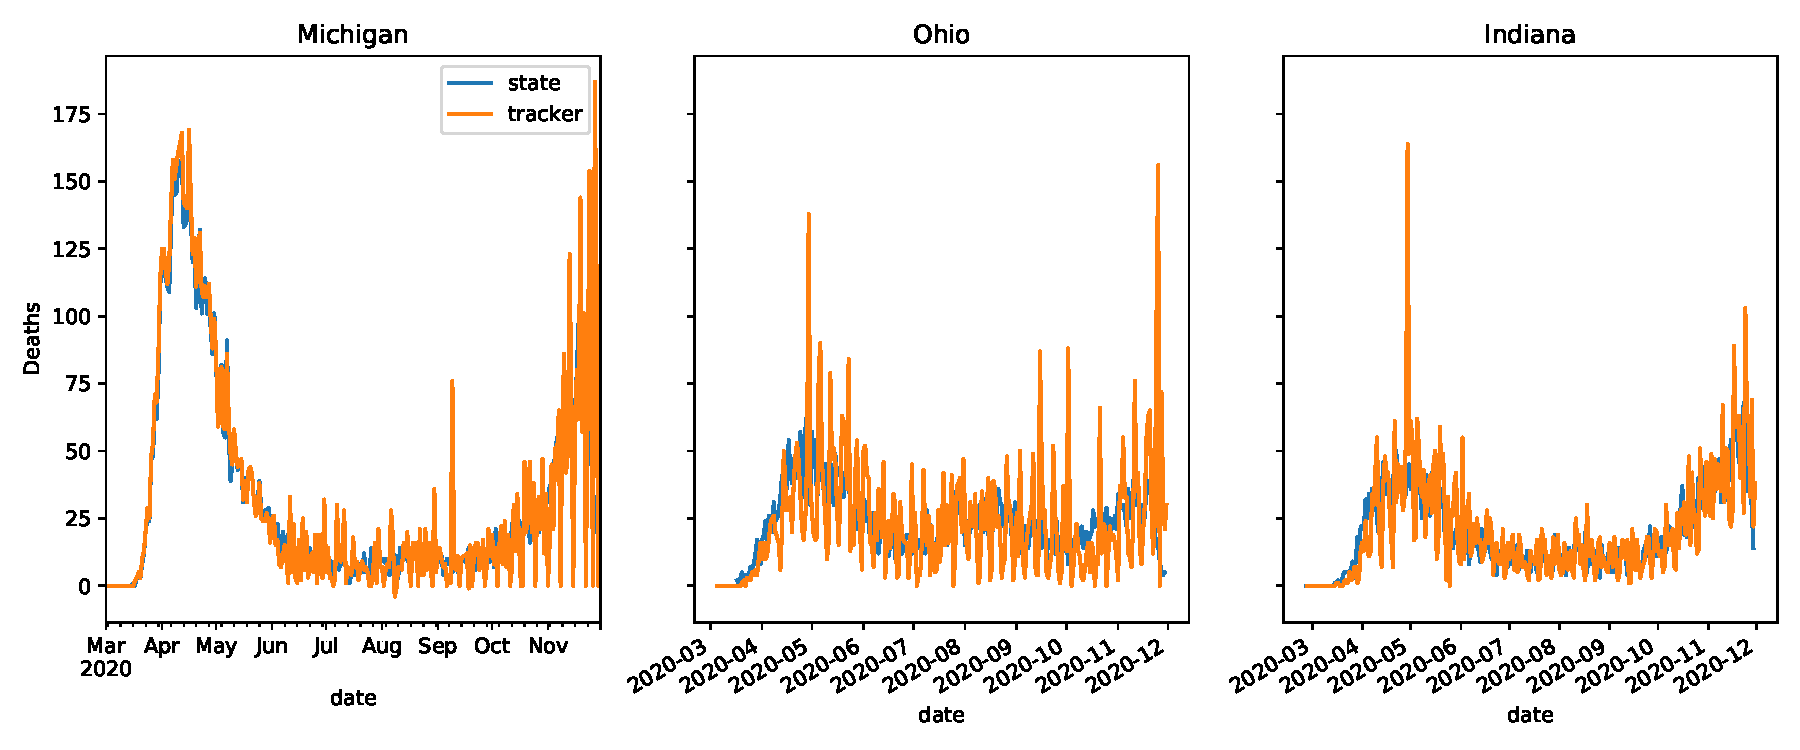
\includegraphics[width=0.45\textwidth]{figs/raw_tracker_comp_nc}
  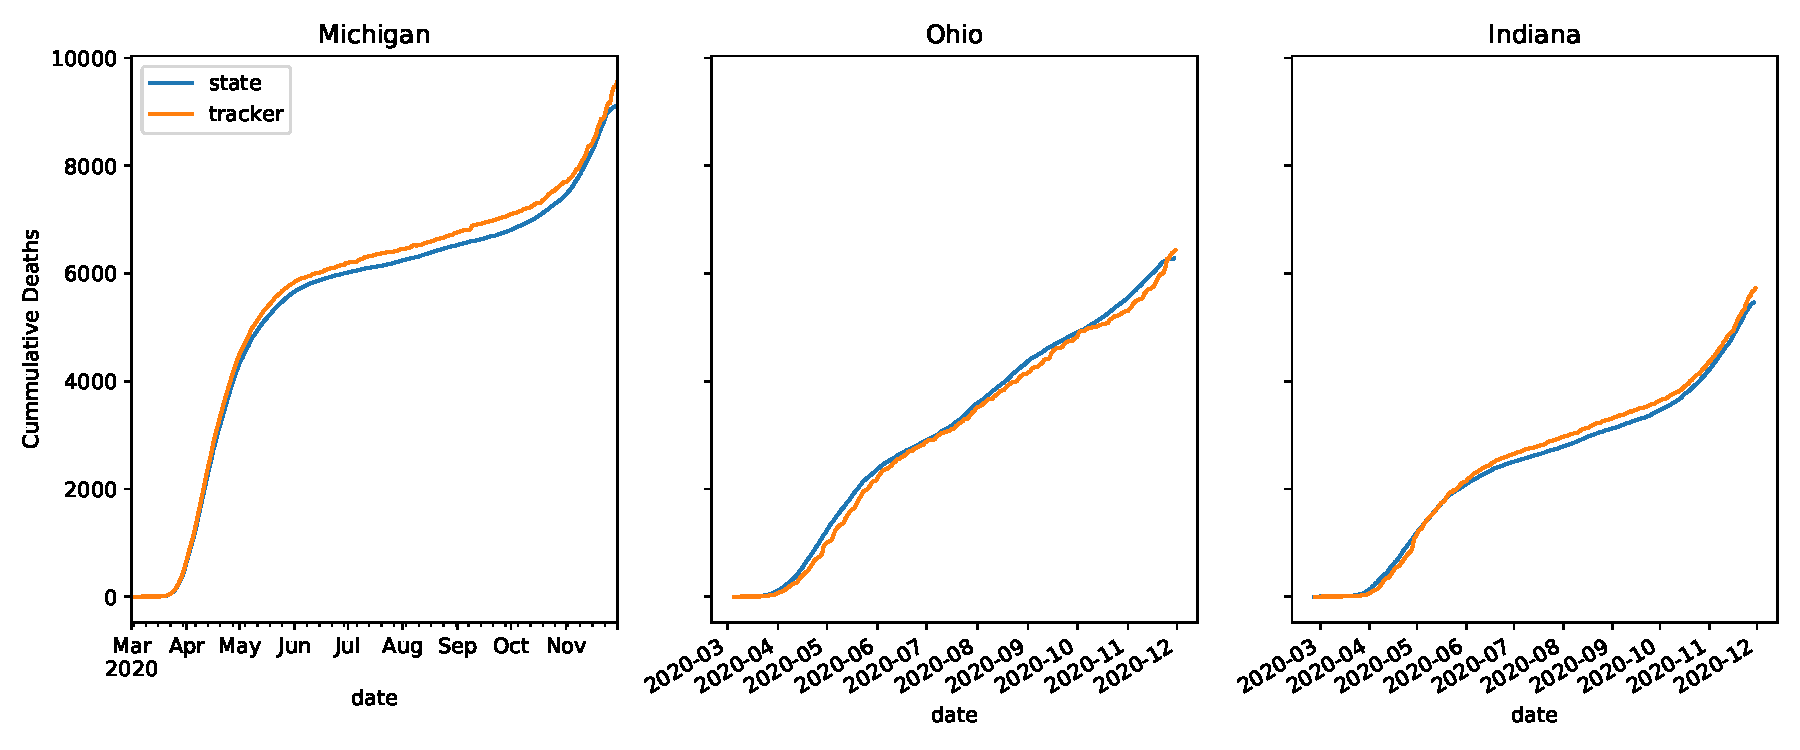
\includegraphics[width=0.45\textwidth]{figs/raw_tracker_comp_cum}
  \caption{Comparison of deaths statistics provided by State Health departments and COVID Tracking Project team. In left and right panes noncumulative and cumulative distributions are shown}
  \label{fig:RT_comp}
\end{figure*}


The main results of our work are presented in figure 4 (see also table \ref{tab:IDC_codes} for the meaning of the codes). For each of the analyzed states you can see weekly distributions of death cases caused by various reasons. As you can see, for all States and for almost all time heart diseases give the main contribution to death statistics. For weeks numbers 15-25 and 45-55, however, contribution of the COVID-19-caused deaths is clearly seen and in some cases (Michigan state, for example) even dominant. It is clear that these two time periods correspond to two waves of the pandemic.


\begin{figure*}
  \centering
  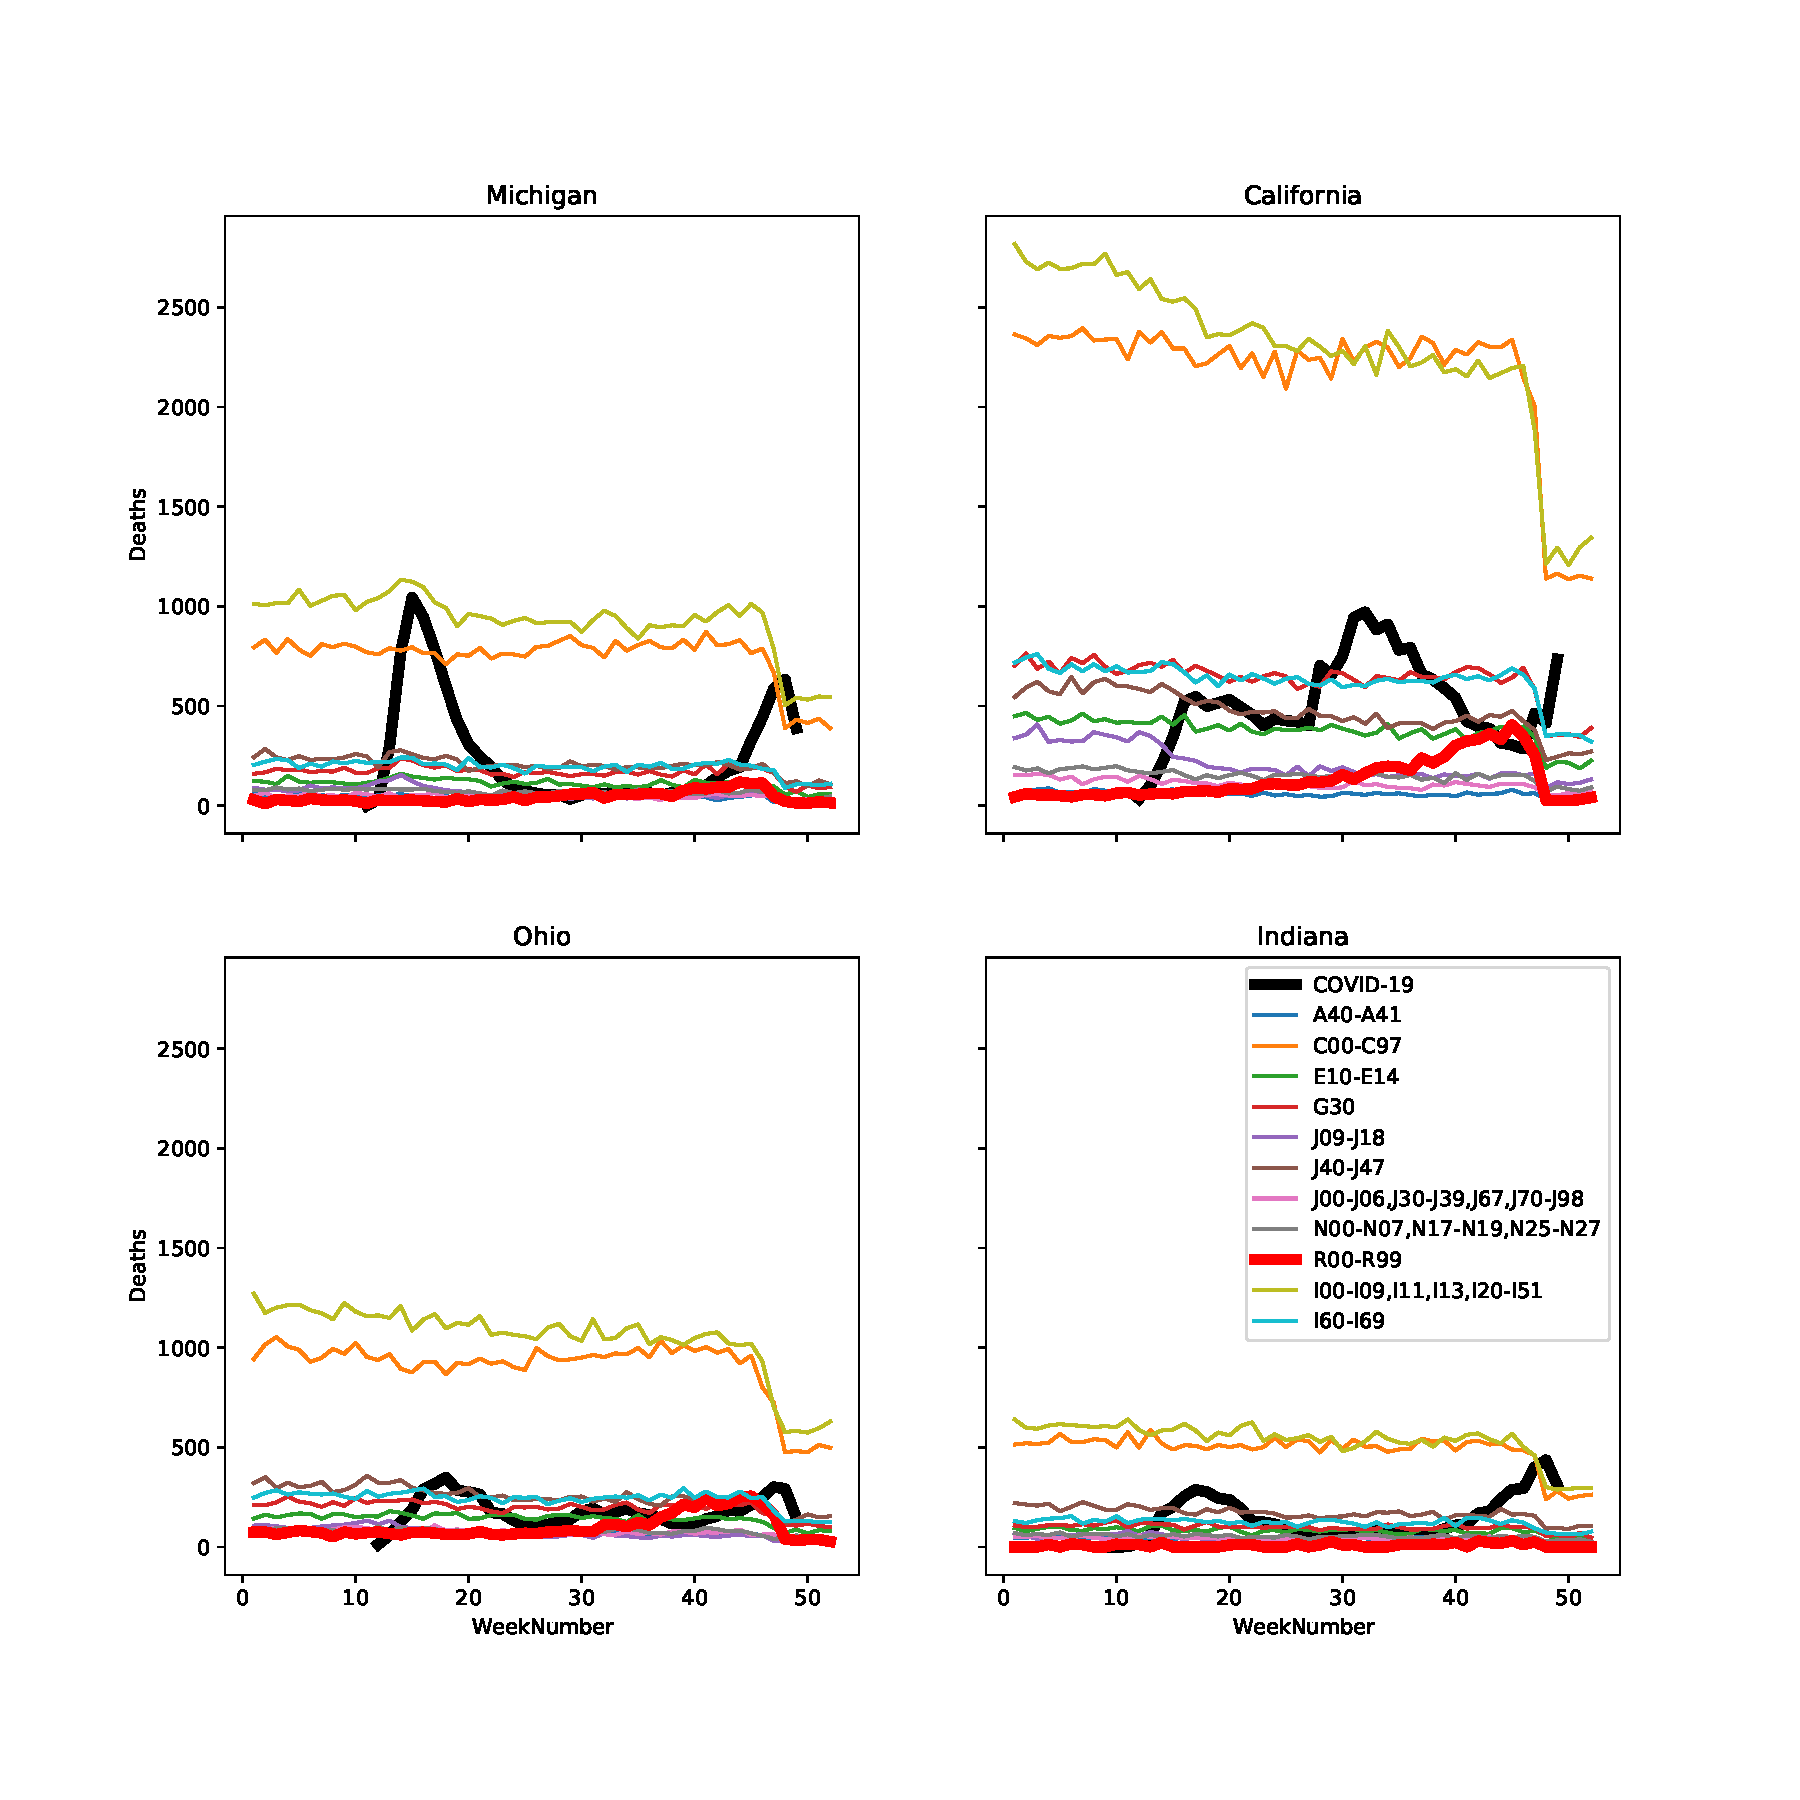
\includegraphics[width=0.9\textwidth]{figs/weekly_deaths}
  \caption{Weekly distribution of deaths by different states and deaths causes}
  \label{fig:weekly_deaths}
\end{figure*}

\begin{table*}
  \centering
  \begin{tabular}{ll}
\toprule
IDC codes&                                              cause \\
\midrule
A40-A41                     &                                        Septicemia  \\
C00-C97                     &                               Malignant neoplasms  \\
E10-E14                     &                                 Diabetes mellitus  \\
G30                         &                                 Alzheimer disease  \\
J09-J18                     &                           Influenza and pneumonia  \\
J40-J47                     &                Chronic lower respiratory diseases  \\
J00-J06,J30-J39,J67,J70-J98 &              Other diseases of respiratory system  \\
N00-N07,N17-N19,N25-N27     &       Nephritis, nephrotic syndrome and nephrosis  \\
R00-R99                     &  Symptoms, signs and abnormal clinical and labo... \\
I00-I09,I11,I13,I20-I51     &                                 Diseases of heart  \\
I60-I69                     &                          Cerebrovascular diseases  \\
\bottomrule
\end{tabular}
\caption{IDC codes from \cite{cdc_international_nodate}}
\label{tab:IDC_codes}
\end{table*}


It could be interesting to study relative role of the virus decease in comparison with other death causes for different states and different time periods. In the case of the Michigan state, for example (see the top left subfigure of figure \ref{fig:weekly_deaths}) the first peak of the pandemic was devastating, the corresponding death rate is comparable  with such as for heart-disease caused cases. The second peak, on the other hand is much more low. The situation is different for Ohio state: during all time period under consideration COVID-19-caused death rates are smaller than for two usual death reasons (heart diseases and neoplasms), but the height of the second mare is comparable with the first one. In the case of the Indiana state the situation is somewhere in the middle.

We can make some assumptions about the reasons of such a difference. As we know, Ohio was one of the first states that have declared the emergency situation and some of the precaution measures were taken in the start of the pandemic. This results in a relatively mild first wave, but the people are too tired from the quarantine, etc, so now we have a serious second mare. In Michigan state the situation is completely different.

There is also the other interesting point in the Ohio and Michigan States data. Starting approximately from week 30 in both cases R00-R99 death cause started to gain mon weights (see red line). According to  International Classification of Diseases scheme  \cite{cdc_international_nodate} these codes correspond to some abnormal symptoms, not elsewhere classified. We do not have enough medical education to make any definite assumptions, but such a behavior exactly during the second wave of a new and not completely studied disease looks rather strange, we can even say suspicions.

% You can see a typical photo of our hero on figure \ref{fig}.

% \begin{figure}[htbp]
% \centerline{
\includegraphics[width = 0.9\columnwidth]{covid19.png}}
% \caption{This is it}
% \label{fig}
% \end{figure}


\section{Conclusion}

It is well known that the ending year is completely different from the others and has changed our life dramatically. we faced a lot of challenges and one of the most famous was the COVID-19 pandemic. Although it started as a small illness in a faraway country on the other side of the ocean, pretty soon the humanity realizes that in this case the situation is very serious. Unlike rather examples (kind flue, swine flue, etc) the the mortality and the virulence of the new one is very high, it cannot be ignored and some precaution measures should be taken.

Such measures were indeed taken, different for different countries and regions. The results of such a measures also varies from countries. The quarantine was introduced throughout the world, various public gatherings and events were canceled (Olympics 2020 in Tokyo, for example), etc. Such actions definitely helped to ease the medical side of the problem, but the other, economical issue arises. Because of the mentioned quarantine a lot of people in the world have lost their jobs, same industries were bankrupted, etc. Moreover, since almost all medical facilities were concentrated on struggle with new disease, less was left for usual, but still important illness, such as heart problems, cancer, etc.

Now a natural question arises: was it worth it? We saved a lot of lives struggling with COVID-19, but a lot of people died since no time and money was left for them because of this struggle. Some analysis should be made to compare all pros and contras of the current situation. This was the main question of our project.

To answer this question we have selected randomly several US States (Ohio, Michigan, Indiana) and searched for statistics of deaths caused by COVID-19 diseases and other, usual reasons. It is clear that huge number of data can be found now concerning CONID, but we were trying to work with the original, raw data, provided by the states themselves. Afterwards we have compared our results with the available processed data. Pretty good qualitative agreement  was observed, although some difference is also visible.

It is interesting to mention that type and quality of this "raw" data depends strongly on the state. Ohio, for example, provides the most rawest from the analyzed states. It means that some efforts should be made to extract some useful information (like time distributions, etc), while the other states give such information directly. On the other hand, the amount of information that can be extracted from the raw data is much higher, than the provided one.

The result of our work can be summarized as follows. On the first sight, if only yearly statistics of deaths is analyzed, the COVID-19 disease does not look very dangerous: in Ohio, for example, is takes the 6th place for death causes between strokes and Alzheimer’s decease. If, however, a more detailed analysis is performed and weekly distributions are considered, the situation changed completely. In such distributions two COVID-19 waves can be seen clearly and on the peaks of these waves the COVID-19 caused death rates are comparable and in some states even higher the the deaths rates caused by most dangerous of the usual issued (heart attacks and cancer). So we can definitely say that taken precaution measures were necessary. The question, however, remains whether we should leave these measures for a long time (for how long?) and  start to return to normal life.

There is one more point that is worth mentioning. In our analysis we have noticed, that in some of the states during the second COVID-19 wave such death cause as “Abnormal symptoms, not elsewhere classified” (IDC codes \# R00-R99) take one of the leading places in the deaths statistics. In Ohio, for example, for several weeks it was in the third place (with first and second being Cancer (IDC \#C00-C97) And Chronic lower respiratory (IDC \#J40-J47) diseases.

% As it was shown in the article \cite{IEEEexample:article_typical}, the night is dark and full of terrors


\bibliographystyle{IEEEtran}
\bibliography{report_litr}

\end{document}

